\documentclass["../Cours.tex"]{subfiles}

\begin{document}
\chapitre{Réciproques}

\partie{Réciproque du théorème de Pythagore}

\theoreme{}{Si, dans un triangle, le carré de la longueur du plus grand côté est égal à la somme des carrés des longueurs des deux autres côtés, alors le triangle est rectangle.}

\exemple{
\begin{center}
    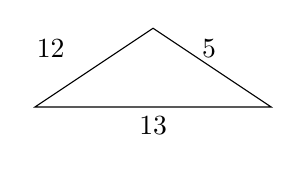
\begin{tikzpicture}
        \draw (0,0) -- (3,0) -- (1.5,1) -- cycle;
        \node[below] at (1.5,0) {13};
        \node[above right] at (2,0.5) {5};
        \node[above left] at (0.5,0.5) {12};
    \end{tikzpicture}
\end{center}
\begin{itemize}
    \item D'une part, $13^2 = 169$\\
    D'autre part, $12^2+5^2 = 144+25=169$
    \item D'après la réciproque du théorème de Pythagore
    \item Le triangle est rectangle
\end{itemize}
}

\partie{Réciproque du théorème de Thalès}

\illustration{
\begin{center}
    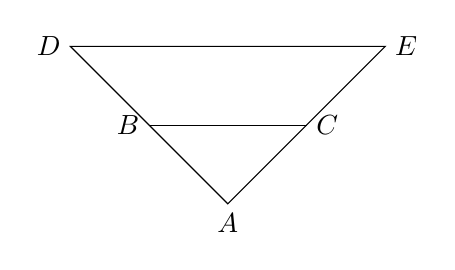
\begin{tikzpicture}
        \draw (0,0) node[below]{$A$} -- (-1,1) node[left]{$B$} -- (-2,2) node[left]{$D$} -- (2,2) node[right]{$E$} -- (1,1) node[right]{$C$} -- cycle;
        \draw (-1,1) -- (1,1);
    \end{tikzpicture}
\end{center}
}

\theoreme{}{Si : 
\begin{itemize}
    \item les points A, B et D sont alignés
    \item les points A, C et E sont alignés
    \item au moins 2 des rapports : $\dfrac{AB}{AD} = \dfrac{AC}{AE} = \dfrac{BC}{DE}$ sont égaux
\end{itemize}
alors les droites $(BC)$ et $(DE)$ sont parallèles.
}

\exemple{
\begin{center}
    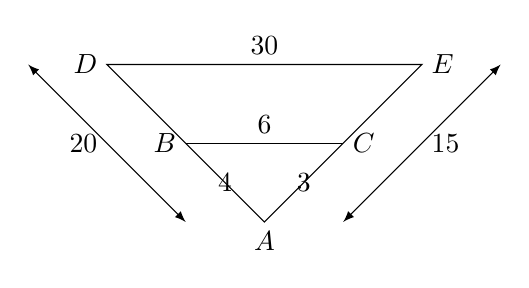
\begin{tikzpicture}
        \draw (0,0) node[below]{$A$} -- (-1,1) node[left]{$B$} -- (-2,2) node[left]{$D$} -- (2,2) node[right]{$E$} -- (1,1) node[right]{$C$} -- cycle;
        \draw (-1,1) -- (1,1);
        \node at (0.5,0.5) {3};
        \node at (-0.5,0.5) {4};
        \draw[latex-latex] (1,0) -- (3,2) node[midway,right,anchor=west]{15};
        \draw[latex-latex] (-1,0) -- (-3,2) node[midway,left,anchor=east]{20};
        \node[above] at (0,2) {30};
        \node[above] at (0,1) {6};
    \end{tikzpicture}
\end{center}
\begin{enumerate}
    \item 
    \begin{itemize}
        \item Les points A, B, D sont alignés
        \item Les points A, C, E sont alignés
        \item D'une part, $\dfrac{AB}{AD} = \dfrac{4}{20} = \dfrac{1}{5}$\\
        D'autre part, $\dfrac{AC}{AE} = \dfrac{3}{15} = \dfrac{1}{5}$
    \end{itemize}
    \item D'après la réciproque du théorème de Thalès
    \item Les droites $(BC)$ et $(DE)$ sont parallèles.
\end{enumerate}
}


\paragraphe{rouge}{Récapitulatif}{
    \textsc{Théorème de Pythagore}\\
    Si 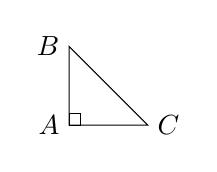
\begin{tikzpicture}
        \draw (0,0) node[left]{$A$} -- (1,0) node[right]{$C$} -- (0,1) node[left]{$B$} -- cycle;
        \draw (0,0) rectangle (0.15,0.15);
    \end{tikzpicture} alors $AB^2+AC^2=BC^2$.\\
    \fbox{Réciproque}\\
    Si $AB^2+AC^2=BC^2$ alors 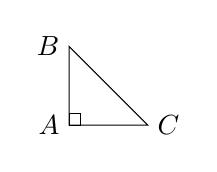
\begin{tikzpicture}
        \draw (0,0) node[left]{$A$} -- (1,0) node[right]{$C$} -- (0,1) node[left]{$B$} -- cycle;
        \draw (0,0) rectangle (0.15,0.15);
    \end{tikzpicture}\\
    \fbox{Contraposée}\\
    Si $AB^2+AC^2\neq BC^2$ alors \begin{tikzpicture}
        \draw (0,0) node[left]{$A$} -- (1,0) node[right]{$C$} -- (0,1) node[left]{$B$} -- cycle;
        \draw (0,0) rectangle (0.15,0.15);
        \draw[rouge] ($(0.075,0.075)+(-0.25,0.25)$) -- ($(0.075,0.075)+(0.25,-0.25)$); 
        \draw[rouge] ($(0.075,0.075)+(-0.25,-0.25)$) -- ($(0.075,0.075)+(0.25,0.25)$); 
    \end{tikzpicture}\\
    \textsc{Théorème de Thalès} 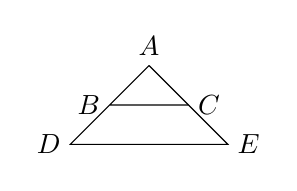
\begin{tikzpicture}
        \draw (0,0) node[above]{$A$} -- (-0.5,-0.5) node[left]{$B$} -- (0.5,-0.5) node[right]{$C$} -- (1,-1) node[right]{$E$} -- (-1,-1) node[left]{$D$} -- cycle;
        \draw (0.5,-0.5) -- (0,0);
    \end{tikzpicture} 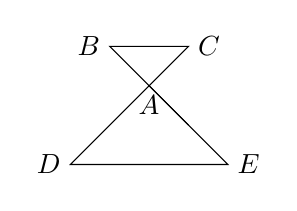
\begin{tikzpicture}
        \draw (0,0) node[below]{$A$} -- (-0.5,0.5) node[left]{$B$} -- (0.5,0.5) node[right]{$C$} -- (-1,-1) node[left]{$D$} -- (1,-1) node[right]{$E$} -- cycle;
        \draw (0.5,-0.5) -- (0,0);
    \end{tikzpicture}\\
    Si $(DE) \paral (BC)$ alors $\dfrac{AD}{AB} = \dfrac{AE}{AC} = \dfrac{DE}{BC}$. 
}



\end{document}